\documentclass{standalone}
\usepackage{pgfplots}
\begin{document}
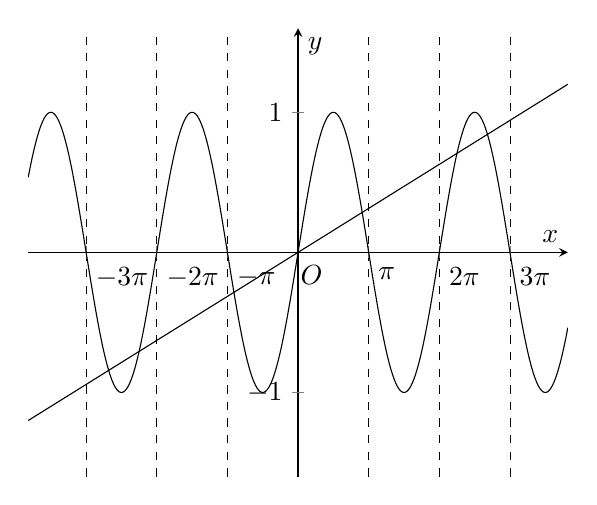
\begin{tikzpicture}
\begin{axis}
[
ymin=-1.6,ymax=1.6,
xmin=-12,xmax=12,
xtick=\empty,
ytick=\empty,
extra x ticks={-9.42478, -6.28319, -3.14159, 3.14159, 6.28319, 9.42478},
extra x tick labels={$-3\pi$, $-2\pi$, $-\pi$, $\pi$, $2\pi$, $3\pi$},
extra y ticks={-1, 1},
extra y tick labels={$-1$, $1$},
every extra x tick/.style={
    xticklabel style={anchor=north west},
    grid=major,
    major grid style={very thin,dashed,black}
},
axis lines = center,
xlabel=$x$,ylabel=$y$,
samples=200,
]
\addplot [black, domain=-12:12, samples=400] {sin(deg(x))};
\addplot [black, domain=-12:12] {x/10};
\node at (axis cs:0.6, -0.16) {$O$} ;
\end{axis}
\end{tikzpicture}
\end{document}
